\chapter{Introduction}\label{chapter:intro}

\begin{figure}[th]
	\centering
		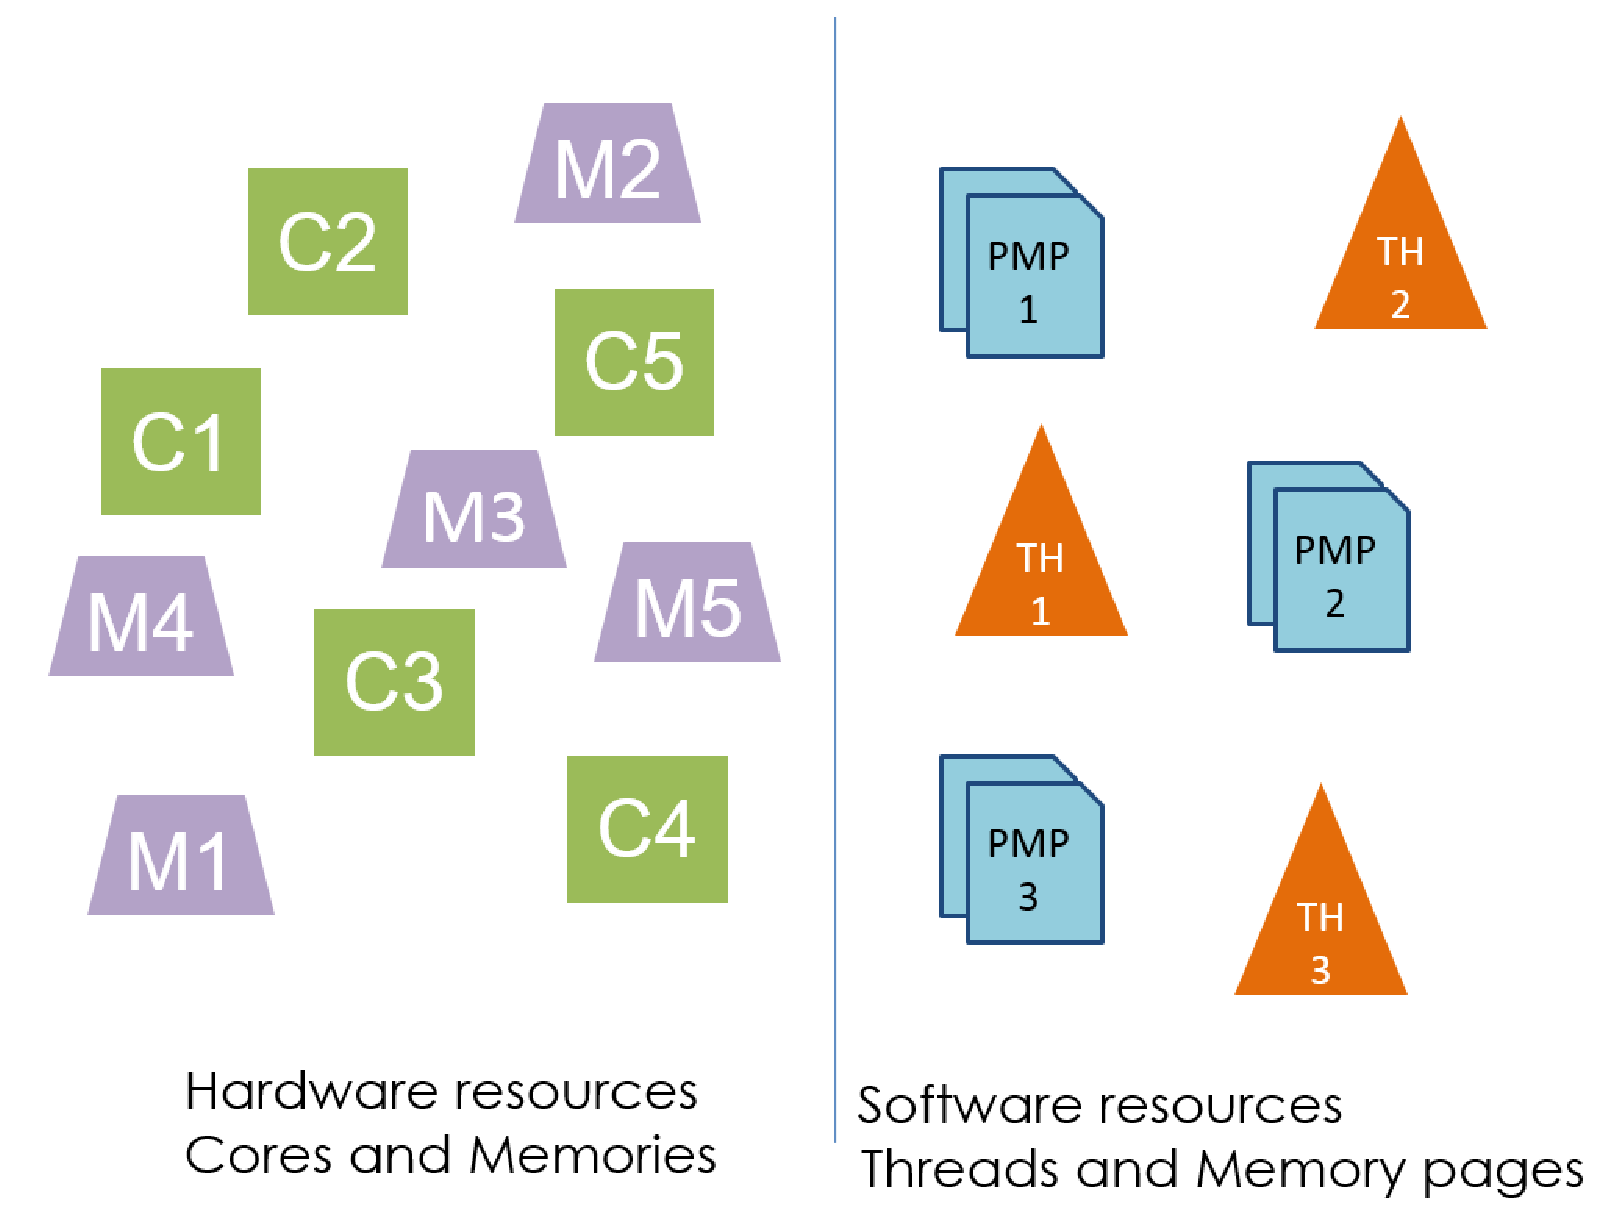
\includegraphics[width=.6\textwidth]{figures/abstract-env.eps}
		\caption[Abstract view of a modern computing environment]{Abstract view of a modern computing environment}
		\label{fig:abstract-cmpenv}
\end{figure}

An abstract representation of a contemporary computing environment is shown in figure \ref{fig:abstract-cmpenv}: The left side consists of computing cores and memories, which are hardware resources and the right hand side shows threads and program memory pages, which are software resources. One of the most challenging goals in computing is to extract the maximum performance possible, which implies the execution of the desired applications with the greatest amount of throughput and the least possible amount of energy usage. For this goal to be achieved, the mapping of the software resources to the hardware resources plays a very important role, this means, which processor executes which threads and which physical memory stores which software memory pages. Another characteristic in today's computing environments is the dynamic makeup of the software resources, which means that the number of resources present in the system change through time and also its nature such as threads being computing bound or memory bound. 

To respond to these challenges, the chair of Computer Architecture and Organization of the Technical University of Munich has developed research which aims to address those requirements: The development of the Autopin and Autopin+ tools deal with the mapping of the threads to CPU cores and the relocation of the threads present on the system in the presence of varying loads. 
With the mapping of the treads to the cores addressed, now the mapping of the program memory pages to the memory modules remains. In NUMA computer systems every processor package has the memory directly attached to it, which helps to increase the access bandwidth and decrease the latency when the accesses originate from the cores present in the chip, but this latency increases when the access originates from one core which belongs to a package different from the one connected to the memory holding the requested page.  The increase in the number of remote accesses might be caused for one of the thread reallocations made by the Autopin tools, and the need to optimize the memory allocation is what leads to the development of the present project.

This document aims to give detail of the development of the sample page migrate tool, or SPM. SPM is a software tool which analyzes the memory access behavior of an observed process by fetching data provide by the processors’ Performance Measurement Unit and based on it reallocates the distribution of the pages if necessary. SPM has two main requirements: First it must support the processors featuring the Intel Sandy Bridge-EP microarchitecture and second its implementation must be made up only of user space code.

The action of the SPM tool is divided into three phases: First, in the observation phase SPM will collect the memory behavior information from the processor’s performance measurement unit, and after a fixed amount of time it will reallocate the pages it seems fit, which happens in the migration phase. Finally in the improved phase it lets the program run until completion and also collects the memory behavior data, but just to facilitate a comparison of the performance with respect to the first phase. In this phase a better performance in comparison to the observed phase is an indicator of the success of the tool.

The SPM tool analyzes the behavior of the observed application in a black box manner, which means that SPM does not have any information about the internals of the observed application and the only information it has is the one provided by the Performance Measurement Units, this means that these units must be tuned to get a fair amount of samples, which is possible by configuring a few parameters that regulate how this units works.

The present document is structured as follows: Chapter \ref{chapter:theorethical} presents the concepts that support the development of the SPM tool. Chapter \ref{chapter:soldesign} presents a deeper description of the performance sampling process in a Linux system and explains in detail the implementation of the SPM tool. Chapter \ref{chapter:envsetup} introduces the characterization of the Intel Sandy Bridge-EP PMU and the benchmarks to be used. Chapter \ref{chapter:res-analysis} presents the results of running the SPM tools together with the distgen and LAMA algorithms and Chapter \ref{chapter:conclusions} presents the conclusions and possibilities of future work.
